%==========================================
%
% Latin.Science 2026  template para artigo
% Adaptado de IEEEtran.cls
%
%==========================================
\documentclass[10pt,conference]{IEEEtran}

% *** CITATION PACKAGES ***
\usepackage{cite}

% *** GRAPHICS RELATED PACKAGES ***
\ifCLASSINFOpdf
   \usepackage[pdftex]{graphicx}
   \DeclareGraphicsExtensions{.pdf,.jpeg,.png,.jpg}
\else
   \usepackage[dvips]{graphicx}
   \DeclareGraphicsExtensions{.eps}
\fi

% *** MATH PACKAGES ***
\usepackage[cmex10]{amsmath}
\interdisplaylinepenalty=2500
\usepackage{amsthm}
\newtheorem{definition}{Definition}

% *** SPECIALIZED LIST PACKAGES ***
\usepackage{algorithmic}

% *** ALIGNMENT PACKAGES ***
\usepackage{array}

% *** SUBFIGURE PACKAGES ***
\ifCLASSOPTIONcompsoc
  \usepackage[caption=false,font=normalsize,labelfont=sf,textfont=sf]{subfig}
\else
  \usepackage[caption=false,font=footnotesize]{subfig}
\fi

% *** PDF, URL AND HYPERLINK PACKAGES ***
\usepackage{url}

% correct bad hyphenation here
\hyphenation{op-tical net-works semi-conduc-tor}

% PACOTES RELACIONADOS A ADIÇÃO DO CABEÇALHO DAS PAGINAS (Template)
\usepackage[left=1.6cm,top=4cm,right=1.6cm,bottom=1.5cm,headheight=1cm]{geometry}
\usepackage{lipsum}
\usepackage{fancyhdr}
\usepackage{tikzpagenodes}

% PACOTES ADICIONADOS PARA SUPORTE AO SEU TEXTO
\usepackage[utf8]{inputenc}
\usepackage[T1]{fontenc}
\usepackage{fontawesome5} % Para os ícones \faDatabase, \faCogs, etc.
\usepackage{float} % Para forçar posição de figuras se necessário

% CONFIGURAÇÕES TIKZ AVANÇADAS (Para o seu diagrama de arquitetura)
\usepackage{tikz}
\usetikzlibrary{calc, positioning, shapes.geometric, arrows.meta, fit, backgrounds}

\renewcommand{\headrulewidth}{0pt}
\renewcommand{\footrulewidth}{0pt}
\pagestyle{fancy}
\setlength\headheight{10.0pt}
\addtolength{\textheight}{-40.0pt}

\fancyhead[L]{\begin{tikzpicture}[remember picture,overlay]
\draw  let \p1=($(current page.north)-(current page header area.south)$),
      \n1={veclen(\x1,\y1)} in
node [inner sep=0,outer sep=0,below right] 
      at (current page.north west){
\includegraphics[width=\paperwidth,height=\n1]{headerimg.png}};
\end{tikzpicture}}

\fancyfoot[R]{\begin{tikzpicture}[remember picture,overlay]
\draw  let \p1=($(current page footer area.north)-(current page.south)$),
      \n1={veclen(\x1,\y1)} in
node [inner sep=0,outer sep=0,above right] 
      at (current page.south west){
\includegraphics[width=\paperwidth,height=\n1]{footerimg.png}};
\end{tikzpicture}}


\begin{document}

% paper title
\title{Dashboard Analítico em R para Visualização Interativa, Modelagem Temporal e Geração de Relatórios Parametrizados Aplicados aos Registros de Licenciamento de Veículos}

%\\[1ex] \Large R Analytical Dashboard for Interactive Visualization, Temporal Modeling and Parameterized Report Generation Applied to Vehicle Licencing Registry

%------------------------------------------------------------------------- 
%------------------------IMPORTANTE---------------------------------------
\newif\iffinal
\finalfalse % <-- MANTIDO FALSE PARA REVISÃO CEGA (BLIND REVIEW)
%------------------------------------------------------------------------- 

%\iffinal
%\else
%  \author{ID do artigo Latin.science 2026: 34563 \\ }
%\fi


\iffinal
\author{
\IEEEauthorblockN{Mário Diego Rocha Valente}
\IEEEauthorblockA{Gerência de Estatística - DETRAN\\
Belém-PA, Brasil\\
mario.valente@detran.pa.gov.br}
\and
\IEEEauthorblockN{Gabriel Baia da Silva}
\IEEEauthorblockA{Faculdade de Computação - UFPA\\
Belém-PA, Brasil\\
gabrielkadran@gmail.com}
\and
\IEEEauthorblockN{Kleber Bezerra Salim}
\IEEEauthorblockA{Gerência de Estatística - DETRAN\\
Belém-PA, Brasil\\
kleber.salim@detran.pa.gov.br}
\and
\IEEEauthorblockN{Tito Félix de Oliveira}
\IEEEauthorblockA{Gerência de Desenvolvimento - DETRAN\\
Belém-PA, Brasil\\
tito.felix@detran.pa.gov.br}
}
\else
%  \author{ID do artigo Latin.science 2026: COLOQUE_SEU_ID_AQUI \\ }
\fi

% make the title area
\maketitle

%utilizado para adicionar header nesta página
\thispagestyle{fancy}

% ===================== RESUMOS (INGLÊS E PORTUGUÊS) =====================

\begin{abstract}
To strengthen evidence-based public policymaking, this paper presents the development of an analytical dashboard in the R programming language for interactive visualization, temporal modeling, and parameterized report generation regarding the vehicle fleet in a Brazilian state. The architecture integrates the \textit{Shiny} and \textit{Quarto Markdown} frameworks, utilizing \textit{Apache Arrow} for data optimization. Predictive modeling for fleet growth up to 2031 compared statistical approaches (ARIMA family) and deep learning methods (LSTM and GRU). The SARIMAX model achieved the best overall fit ($R^2 = 0.7240$), while the GRU model presented the lowest predictive error ($MAPE = 5.19\%$). To ensure scalability and high availability, a \textit{DevOps} workflow based on containerization and orchestration (\textit{Podman}, GitLab CI/CD, and \textit{Kubernetes}) was implemented. The project highlights the feasibility of combining data science, machine learning, and modern orchestration to support government management and public transparency.
\end{abstract}

\renewcommand{\IEEEkeywordsname}{Keywords}
\begin{IEEEkeywords}
Analytical Dashboard; Interactive Visualization; Temporal Series; Predictive Modeling; Deep Learning; Public Transparency.
\end{IEEEkeywords}

\renewcommand{\abstractname}{Resumo}
\begin{abstract}
Para fortalecer a formulação de políticas públicas baseadas em evidências, este trabalho apresenta o desenvolvimento de um dashboard analítico em linguagem R para a visualização interativa, modelagem temporal e geração de relatórios parametrizados da frota veicular de um estado brasileiro. A arquitetura integra os \textit{frameworks Shiny} e \textit{Quarto Markdown}, utilizando \textit{Apache Arrow} para otimização de dados. A modelagem preditiva do crescimento da frota até 2031 comparou abordagens estatísticas (família ARIMA) e de aprendizado profundo (LSTM e GRU). O modelo SARIMAX obteve o melhor ajuste global ($R^2 = 0,7240$), enquanto o GRU apresentou o menor erro preditivo ($MAPE = 5,19\%$). Para assegurar escalabilidade e alta disponibilidade, implementou-se um fluxo \textit{DevOps} baseado em conteinerização e orquestração (\textit{Podman}, GitLab CI/CD e \textit{Kubernetes}). O projeto evidencia a viabilidade de unir ciência de dados, aprendizagem de máquina e orquestração moderna no apoio à gestão governamental e transparência pública.
\end{abstract}

\renewcommand\IEEEkeywordsname{Palavras-chave}
\begin{IEEEkeywords}
Dashboard Analítico; Visualização Interativa; Séries Temporais; Modelagem Preditiva; Aprendizado Profundo; Transparência Pública.
\end{IEEEkeywords}

\IEEEpeerreviewmaketitle

% ===================== CORPO DO ARTIGO =====================

\section{Introdução}

O crescimento acelerado da produção de dados governamentais tem ampliado a necessidade de mecanismos capazes de transformar grandes volumes de informações em instrumentos eficazes de transparência pública, apoio à tomada de decisão e formulação de políticas públicas baseadas em evidências \cite{janssen2012}. No contexto da administração pública brasileira, iniciativas voltadas à abertura e disseminação de dados passaram a ganhar maior relevância após a promulgação da Lei de Acesso à Informação (Lei nº 12.527/2011), estabelecendo diretrizes para disponibilização ativa de informações institucionais à sociedade \cite{brasil2011}.


Segundo o Radar Nacional da Transparência Pública \cite{atricon2025}, embora os índices de transparência tenham apresentado evolução significativa nos últimos anos, ainda existem lacunas relacionadas à disponibilização estruturada de informações analíticas em diversos setores governamentais, especialmente em áreas relacionadas à mobilidade urbana e gestão do trânsito. Nesse cenário, órgãos executivos de trânsito passaram a demandar soluções computacionais capazes de integrar processamento estatístico, visualização interativa e disseminação automatizada de informações em ambientes acessíveis ao público externo.

A crescente complexidade dos ambientes analíticos contemporâneos impulsionou a adoção de plataformas integradas para ciência de dados e visualização interativa. Tradicionalmente, ferramentas de \textit{Business Intelligence }(BI) proprietárias têm sido adotadas por instituições públicas. No entanto, essas soluções frequentemente esbarram em limitações de customização, algoritmos \textit{black-box} e altos custos de licenciamento e \textit{vendor lock-in} (dependência de fornecedor). Esse panorama motivou uma maior aproximação entre análise estatística robusta e desenvolvimento de sistemas web de código aberto \cite{wickham2017}. 

Nesse contexto, a linguagem R destaca-se por sua ampla utilização em aplicações estatísticas, mineração de dados e construção de aplicações analíticas reativas \cite{chang2026}. Paralelamente, frameworks como Shiny possibilitam o desenvolvimento de dashboards interativos sem a necessidade de implementação tradicional em múltiplas linguagens de front-end e back-end, garantindo a integração nativa com modelos de inteligência artificial de ponta.

No estado em estudo, um órgão de trânsito administra uma base de dados veiculares associada ao Registro Nacional de Veículos Automotores (RENAVAM), composta por milhões de registros históricos. A elevada dimensionalidade dessas informações espaço-temporais, associada à necessidade de indicadores de motorização e projeções preditivas, torna indispensável a utilização de arquiteturas analíticas escaláveis. O desafio se acentua ao lidar com dados de cidades do interior, onde a esparsidade dos registros históricos exige técnicas avançadas de engenharia de \textit{features} e \textit{deep learning} para garantir a convergência de modelos \cite{knaflic2019storytelling}.

Antes do desenvolvimento desta solução, solicitações estatísticas veiculares eram atendidas manualmente, resultando em elevada demanda operacional e lentidão na disseminação contínua de informações. A ausência de ferramentas interativas restringia a exploração dinâmica por gestores públicos, pesquisadores e cidadãos interessados em compreender os padrões de crescimento e distribuição da frota veicular.


Diante desse contexto, este trabalho apresenta o desenvolvimento de um sistema analítico integrado baseado na linguagem R, utilizando Shiny e Quarto para a construção de dashboards interativos e geração de relatórios parametrizados sobre a frota desse órgão. A arquitetura incorpora ETL otimizado via formato colunar Apache Arrow \cite{richardson2026}, modelagem estatística de séries temporais, redes neurais e integração contínua baseada em orquestração de microsserviços \cite{burns2016borgomega}.

No componente analítico, empregaram-se modelos da família ARIMA \cite{box1970time}, com variáveis exógenas (SARIMAX), além de arquiteturas baseadas em Redes Neurais Recorrentes, como \textit{Long Short-Term Memory} (LSTM) \cite{hochreiter1997} e \textit{Gated Recurrent Unit} (GRU). A geração automatizada de documentos em Quarto Markdown ampliou a capacidade de disseminação de informações técnicas por município e categoria veicular, assegurando reprodutibilidade computacional \cite{xie2018}.

A solução desenvolvida também incorpora práticas de \textit{DevOps} voltadas à ciência de dados (MLOps), integrando conteinerização (\textit{Podman}), \textit{pipelines} (GitLab CI/CD) e orquestração (\textit{Kubernetes}), garantindo escalabilidade em ambiente de nuvem governamental \cite{humble2010, burns2016borgomega}.

O objetivo central deste trabalho é desenvolver uma arquitetura analítica integrada para disponibilização pública de estatísticas da frota veicular. Como contribuição adicional, o trabalho demonstra, de forma inédita na literatura nacional, a viabilidade de integrar os \textit{framework} (\texttt{Arrow}, \texttt{Shiny}, \texttt{Quarto} e \texttt{Keras/TensorFlow}) sob governança de \textit{Kubernetes} no apoio à transparência pública de dados de mobilidade.


%------------------------------------------------------------------------------
\section{Trabalhos Relacionados}

O uso de plataformas analíticas interativas voltadas à transparência pública e exploração de dados governamentais tem crescido significativamente, impulsionado pelas iniciativas de governo digital \cite{janssen2012}. Nesse cenário, dashboards analíticos passaram a desempenhar um papel estratégico.

Diversos estudos têm explorado o Shiny em contextos governamentais. Kuo et al. \cite{kuo2019} desenvolveram um dashboard interativo para monitoramento epidemiológico utilizando dados espaciais e séries temporais em R, demonstrando como aplicações reativas ampliam a disseminação em tempo real. Fay et al. \cite{fay2021} destacam o potencial do Shiny na construção de plataformas reprodutíveis, enfatizando a integração com bibliotecas estatísticas. Contudo, em aplicações de mobilidade pública, o desafio do volume de dados em memória frequentemente inviabiliza arquiteturas Shiny tradicionais que não utilizem esquemas \textit{out-of-memory}.


No domínio da mobilidade urbana, Wang et al. \cite{wang2020} utilizaram séries temporais para previsão do crescimento automotivo em centros urbanos, evidenciando a importância preditiva no planejamento viário. Em abordagens administrativas, Barros et al. \cite{barros2017} discutem o uso de ARIMA e SARIMA em dados com sazonalidade e tendência. Mais recentemente, modelos de aprendizado profundo (LSTM e GRU) vêm sendo aplicados a séries temporais complexas \cite{ghojogh2023recurrentneuralnetworkslong}, apresentando excelente desempenho ao capturar dependências não lineares e múltiplos fatores externos.

Além da camada analítica, a reprodutibilidade computacional tem sido uma barreira. Ferramentas como Quarto e R Markdown integram código e texto paramétrico \cite{xie2018}. Na esfera da infraestrutura analítica escalável, a engenharia de software voltada a dados (\textit{DataOps} / MLOps) tornou-se imperativa \cite{humble2010}. Tecnologias como Kubernetes \cite{burns2016borgomega} garantem isolamento, escalabilidade e alta disponibilidade de modelos de \textit{machine learning} expostos via interfaces interativas.

Embora existam trabalhos sobre dashboards em R, observa-se uma carência de arquiteturas na literatura científica que integrem simultaneamente: processamento \textit{lazy-loading} colunar, visualização interativa, previsão por aprendizado profundo e \textit{deployment} escalável via Kubernetes no escopo de departamentos de trânsito. Este trabalho supre tal lacuna ao consolidar uma esteira analítica governamental completa.

%---------------------------------------------------------------------------%

\section{Materiais e Métodos}

A aplicação web foi desenvolvida integralmente no ecossistema R. A sua escolha justifica-se pela aderência unificada a todo o ciclo de vida do dado: desde as extrações via APIs, modelagem estatística, inferência via grafos computacionais (com \textit{TensorFlow} no \textit{backend}), até o delineamento da interface web. Os dados têm como origem o banco relacional interno do órgão, gerido pelo setor de tecnologia.

\subsection{Arquitetura de Dados Otimizada com Apache Arrow e Parquet}

O processo de Extração, Transformação e Carga (ETL) foi implementado utilizando o pacote \texttt{tidyverse} \cite{tidyverse2019}, responsável pela sanitização, estruturação e padronização geométrica da base. Para lidar com a volumetria massiva sem incorrer em gargalos de memória RAM do servidor R, as tabelas originais foram transmutadas para o formato colunar \texttt{.parquet} e orquestradas pelo \textit{framework} \texttt{arrow} \cite{arrow2026}. 

A utilização do Apache Arrow possibilita leituras do tipo \textit{zero-copy} e operações de \textit{lazy loading}. Isso significa que consultas analíticas realizadas via \texttt{dplyr} \cite{dplyr2026} como filtragens demográficas temporais (\texttt{filter}, \texttt{group\_by}) são convertidas em planos de execução otimizados diretamente no disco (pushdown de predicados), subindo para a memória apenas o vetor resultante estritamente necessário para a plotagem gráfica do usuário, conferindo altíssima responsividade ao \textit{dashboard}.

\subsection{Interface e Reatividade Web}

A aplicação utiliza o \textit{framework Shiny} organizado no padrão \textit{User Interface} (UI) e \textit{Server}. A UI utiliza o pacote \texttt{bs4Dash} (baseado em Bootstrap 4) para prover responsividade tátil em dispositivos móveis. O componente servidor rege os grafos de reatividade estatística. O sistema conta com tabelas dinâmicas renderizadas em React.js via \texttt{reactable} \cite{reactable2026}, integração de geoprocessamento em mapas coropléticos poligonais (\texttt{leaflet} \cite{leaflet2025}) e séries interativas vetorizadas (\texttt{echarts4r} \cite{echarts4r2026}). O macrofluxo estrutural é delineado na Fig.~\ref{fig:arquitetura}.

\begin{figure}[!ht]
\centering
\resizebox{\columnwidth}{!}{%
\begin{tikzpicture}[
    node distance=0.5cm and 1.6cm,
    box/.style={draw, rounded corners = 3pt, rectangle, minimum width=2.5cm, minimum height=0.85cm, align=center, font=\small},
    db/.style={draw, cylinder, shape border rotate=90, aspect=0.25, minimum width=2.5cm, minimum height=0.85cm, align=center, font=\small},
    arrow/.style={-Stealth, thick}, 
    barrow/.style={Stealth-Stealth, thick},
    darrow/.style={-Stealth, dashed}
]
%% COLUNA 1 — Preparação de Dados
\node[db] (A) {\Large\faDatabase\\[4pt] Fontes de Dados\\{\footnotesize (.csv/.xls)}};
\node[box, below=of A] (B) {\Large\faCogs\\[4pt] Processamento ETL\\{\footnotesize (\textit{Tidyverse})}};
\node[db,  below=of B] (C) {\Large\faBolt\\[4pt] Dados Otimizados\\{\footnotesize (\textit{Arrow / Parquet})}};
\draw[arrow] (A) -- (B);
\draw[arrow] (B) -- (C);
\begin{scope}[on background layer]
  \node[draw, dashed, inner sep=0.3cm, fit=(A)(B)(C),
        label={[font=\footnotesize]above:Preparação de Dados}] (box1) {};
\end{scope}

%% COLUNA 2 — Aplicação R / Shiny
\node[box, right=1.8cm of B] (D) {\Large\faServer\\[4pt] Motor Reativo (dplyr)\\{\footnotesize Lógica do Servidor}};
\node[box, above right=0.4cm and 1.2cm of D] (E) {\Large\faChartLine\\[4pt] Modelagem\\{\footnotesize ARIMA / GRU}};
\node[box, right=1.2cm of D]                 (F) {\Large\faDesktop\\[4pt] Interface UI\\{\footnotesize bs4Dash}};
\node[box, below right=0.4cm and 1.2cm of D] (G) {\Large\faChartBar\\[4pt] Visualizações\\{\footnotesize echarts4r / leaflet}};
\draw[barrow] (D) -- (E);
\draw[arrow] (D) -- (F);
\draw[arrow] (D) -- (G);
\begin{scope}[on background layer]
  \node[draw, dashed, inner sep=0.3cm, fit=(D)(E)(F)(G),
        label={[font=\footnotesize]above:Camada de Aplicação R -- Shiny}] (box2) {};
\end{scope}

%% COLUNA 3 — Saída e Hospedagem
\node[box, right=1.2cm of F] (H) {\Large\faGlobe\\[4pt] Renderização\\{\footnotesize Navegador Web}};
\node[db,  below=of H]       (I) {\Large\faCubes\\[4pt] Produção DevOps\\{\footnotesize \textit{Podman/Kubernetes}}};
\begin{scope}[on background layer]
  \node[draw, dashed, inner sep=0.3cm, fit=(H)(I),
        label={[font=\footnotesize]above:Saída e Hospedagem}] (box3) {};
\end{scope}

%% CONEXÕES ENTRE COLUNAS
\draw[arrow] (C.east) -- ++(1,0) coordinate (ElbowLL) -- (D.west);
\node[below=2pt, font=\scriptsize] at (ElbowLL) {Lazy Loading};

\draw[arrow] (F) -- (H);
\draw[arrow] (G) -- (H);

%% Deploy
\draw[arrow] (box2.south) -- ++(0,-1.4) -|
              node[below, font=\scriptsize, pos=0.25]{Pipeline CI/CD} (I.south);
\end{tikzpicture}%
}
\caption{Arquitetura estendida do sistema: do processamento lógico e armazenamento colunar à implantação interativa.}
\label{fig:arquitetura}
\end{figure}


%----------------------------------------------------------------------------------%

\section{Modelagem Estatística e Deep Learning}

Adotou-se a abordagem de \textit{storytelling} analítico de Knaflic (2019) para projetar os dados espacialmente e temporalmente. As seções a seguir fundamentam os algoritmos preditivos empregados. 

\subsection{Modelos Estatísticos Clássicos (Família ARIMA)}
Os modelos estatísticos clássicos pertencentes à família ARIMA são amplamente empregados por sua capacidade nativa de absorver tendências seculares e padrões de autocorrelação \cite{box1970time}. O modelo base $\textbf{ARIMA(p,d,q)}$ é dado por~(\ref{eq:arima}).

\begin{equation}
\phi(L)\Delta^{d} y_{t} = \theta(L)\varepsilon_{t}
\label{eq:arima}
\end{equation}

Em que $\phi(L)$ e $\theta(L)$ representam, respectivamente, os componentes autorregressivo e de médias móveis, cujas ordens são dadas por $p$ e $q$; $d$ é o grau de diferenciação integrativa, $L$ é o operador de defasagem e $\varepsilon_t$ representa o ruído branco. A sazonalidade de 12 meses observada na arrecadação de IPVA e licenciamentos é tratada no $SARIMA(p,d,q)(P,D,Q)_{12}$, Equação~(\ref{eq:sarima}).

\begin{equation}
\phi(L)\Phi(L^{12})\Delta^{d}\Delta_{12}^{D} y_{t} = \theta(L)\Theta(L^{12})\varepsilon_{t}
\label{eq:sarima}
\end{equation}

Em que $\Phi(L^{12})$ e $\Theta(L^{12})$ representam os componentes sazonais autorregressivo e de médias móveis, cujas ordens são dadas por $P$ e $Q$, enquanto $D$ corresponde ao grau de diferenciação sazonal.

Para mitigação de anomalias econômicas, aplicou-se o modelo avançado $SARIMAX(p,d,q)(P,D,Q)_{12}$, Equação~(\ref{eq:sarimax}), que incorpora uma matriz de regressores exógenos ($X_t$).

\begin{equation}
\phi(L)\Phi(L^{12})\Delta^{d}\Delta_{12}^{D} y_{t} = \theta(L)\Theta(L^{12})\varepsilon_{t} + \beta X_{t}
\label{eq:sarimax}
\end{equation}

O vetor $X_t$ modelou de forma exógena as retrações macroeconômicas sofridas pelo Brasil (2013--2017), servindo como intervenção de "pulso" para garantir a estabilidade assintótica a longo prazo.

\subsection{Redes Neurais Recorrentes e Modelagem Tensorial (GRU)}

Para a captura de não linearidades severas de longo alcance, projetaram-se arquiteturas de \textit{Deep Learning}: \textbf{LSTM} (\textit{Long Short-Term Memory}) e \textbf{GRU} (\textit{Gated Recurrent Unit}). A implementação utilizou \texttt{keras} e \texttt{tensorflow} via R, otimizada com Adam e backpropagation-through-time (BPTT).

\begin{figure}[!ht]
    \centering
    \subfloat[Célula LSTM]{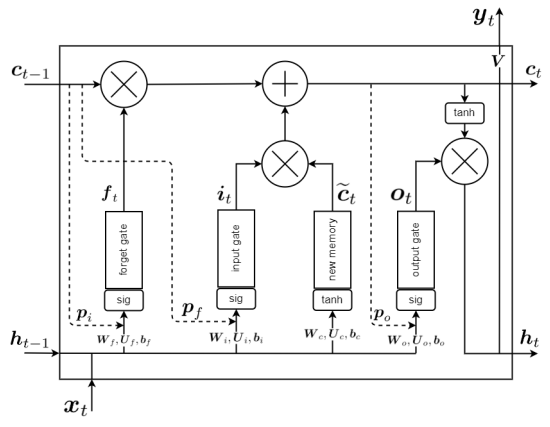
\includegraphics[width=1.8in]{LSTM.png}\label{fig:lstm}}
    \hfil
    \subfloat[Célula GRU]{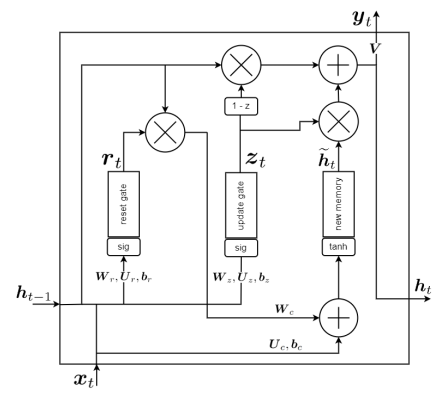
\includegraphics[width=1.6in]{GRU.png}\label{fig:celula_gru}}
    \caption{Representação das arquiteturas de Redes Neurais Recorrentes \cite{ghojogh2023recurrentneuralnetworkslong}.}
    \label{fig:redes_neurais}
\end{figure}

\newpage
Redes neurais recorrentes convencionais frequentemente esbarram na limitação do gradiente descendente (\textit{vanishing gradient}), o que dificulta o aprendizado de dependências temporais extensas. A arquitetura LSTM resolve esse problema introduzindo mecanismos de controle de fluxo de informação chamados de portões (\textit{gates}): o portão de esquecimento (\textit{forget gate}), responsável por descartar dados irrelevantes; o portão de entrada (\textit{input gate}), que assimila novas informações à memória; e o portão de saída (\textit{output gate}), responsável por transmitir os valores processados para os estados subsequentes da rede \cite{hochreiter1997}.

Enquanto a LSTM possui um custo computacional maior devido ao uso constante desses três \textit{gates}, a GRU otimiza significativamente esse processo fundindo os estados ocultos e utilizando apenas dois mecanismos principais: o portão de atualização (\textit{update gate}) e o portão de redefinição (\textit{reset gate}) \cite{cho2014learning}. Para formalizar a dinâmica de aprendizado da célula GRU, que obteve o melhor desempenho neste estudo, o fluxo de informação no instante $t$ é governado pelas seguintes equações:

$$z_t = \sigma(W_z x_t + U_z h_{t-1} + b_z)$$
$$r_t = \sigma(W_r x_t + U_r h_{t-1} + b_r)$$
$$\tilde{h}_t = \tanh(W_h x_t + U_h (r_t \odot h_{t-1}) + b_h)$$
$$h_t = (1 - z_t) \odot h_{t-1} + z_t \odot \tilde{h}_t$$

Onde $\sigma$ denota a função de ativação sigmoide não linear, $\odot$ representa o produto de Hadamard (\textit{element-wise}), $x_t$ é o vetor de entrada multivariado, $h_{t-1}$ é o estado oculto da iteração anterior. As matrizes de pesos $W$ e $U$, bem como os vetores de viés $b$, constituem os parâmetros hiperdimensionais otimizados iterativamente pelo otimizador Adam durante a fase de convergência.

\newpage
Para resolver o problema prático de ausência de granularidade temporal nas cidades do interior do estado (esparsidade de amostras), este trabalho propõe uma abordagem de \textbf{engenharia de tensores multidimensionais}, ilustrada na Fig.~\ref{fig:gru_fluxo}.

\begin{figure}[!ht]
\centering
\resizebox{\columnwidth}{!}{%
\begin{tikzpicture}[
    node distance=1cm and 1.2cm,
    box/.style={draw, rectangle, rounded corners=4pt, minimum width=2.8cm, minimum height=1.5cm, align=center, font=\small},
    arrow/.style={-Stealth, thick, color=black!80}
]
% Nodes
\node[box, fill=blue!10, draw=blue!40] (tensor) {\textbf{Tensor de Entrada 3D}\\ {\scriptsize (Modelagem de Dados)}\\[6pt] \footnotesize $[Amostras \times Passos \times Variáveis]$ \\ \footnotesize $(M \times 24 \times N)$};

\node[box, right=of tensor, fill=green!10, draw=green!50] (gru) {\textbf{Camada GRU}\\ \footnotesize Extração de Padrões\\ \footnotesize Espaço-Temporais Ocultos};

\node[box, right=of gru, fill=orange!10, draw=orange!50] (dense) {\textbf{Camada Densa}\\ \footnotesize Recombinação Linear\\ \footnotesize (Função de Ativação Linear)};

\node[box, right=of dense, fill=red!10, draw=red!40] (output) {\textbf{Vetor de Saída}\\ \footnotesize Previsão $t+h$\\ \footnotesize (Municípios Consolidados)};

% Arrows
\draw[arrow] (tensor) -- node[above, font=\scriptsize] {\textit{Batching}} (gru);
\draw[arrow] (gru) -- node[above, font=\scriptsize] {$H_{t}$} (dense);
\draw[arrow] (dense) -- (output);
\end{tikzpicture}%
}
\caption{Esquema da modelagem de dados para o algoritmo GRU empregado.}
\label{fig:gru_fluxo}
\end{figure}

Em vez de instanciar dezenas de modelos independentes para cada município (o que sobrecarregaria a infraestrutura e impediria a convergência de cidades pequenas), optou-se por uma decomposição tensorial. Primeiramente, estabilizou-se a variância e a escala das curvas através da normalização Z-score em cada vetor municipal, dada por:

$$z = \frac{x - \mu}{\sigma}$$

Onde $\mu$ é a média histórica e $\sigma$ é o desvio padrão da frota do município. Após essa etapa geométrica, os vetores padronizados foram acoplados aos \textit{lags} temporais, originando uma matriz de $N$ colunas. Esse arranjo estrutural resulta num \textit{tensor de entrada global} tridimensional. Essa topologia força a camada densa da GRU a transferir a \textit{feature representation} dos padrões de crescimento de grandes polos urbanos para mitigar as dinâmicas escassas de municípios menores.

%-------------------------------------------------------------------------------%
\subsection{Subsistema de Relatórios Parametrizados (Quarto)}

O ecossistema analítico culmina na geração automatizada de documentos. O servidor \textit{Shiny} intercepta as coordenadas de filtros (espaço, tempo e tipologia) inseridas pelo usuário na UI e as encapsula nos metadados YAML de um documento mestre Quarto Markdown (\texttt{.qmd}) via argumento \texttt{params}. 

Isso força a execução isolada de uma \textit{thread} R no \textit{background} que realiza consultas otimizadas via \textit{arrow}. O Quarto compila gráficos vetorizados (via \texttt{ggplot2}) e tabelas gramaticais (via \texttt{gt}), transmutando-os em código \LaTeX{}. Acoplado a um preâmbulo institucional de geometria e identidade visual (\texttt{HEADER.tex}), o motor \textit{TinyTeX} gera um PDF de altíssima fidelidade e o retorna via \textit{download} no front-end, eliminando a dependência manual de elaboração de boletins gerenciais e mitigando falhas humanas na prestação de contas governamental.

%-------------------------------------------------------------------------------%
\subsection{Metodologia de Deployment e Integração Contínua}

Para garantir resiliência e alta disponibilidade, implementou-se um fluxo \textit{DevOps} e CI/CD (Integração/Entrega Contínuas), ilustrado na Fig.~\ref{fig:deployment}. O ecossistema \textit{Podman} \cite{podman2026} atua na criação da imagem imutável do sistema operacional Linux que embala o código R, suas dependências sistêmicas (C++) e o código fonte. 

\begin{figure}[!ht]
\centering
\resizebox{\columnwidth}{!}{%
\begin{tikzpicture}
[
    node distance=0.8cm and 1.8cm,
    box/.style={draw, rounded corners = 3pt, rectangle, minimum width=2.8cm, minimum height=1.2cm, align=center, font=\footnotesize},
    db/.style={draw, cylinder, shape border rotate=90, aspect=0.25, minimum width=2.8cm, minimum height=1.2cm, align=center, font=\footnotesize},
    arrow/.style={-Stealth, thick}, 
    barrow/.style={Stealth-Stealth, thick},
    darrow/.style={-Stealth, dashed}
]

%% 1. NÓS INTERNOS
\node[box] (scripts) {
\includegraphics[height=0.8cm]{R.jpg} \\[4pt] ~ \texttt{(App.R)}};
\node[box, below=of scripts] (docker) {
\includegraphics[height=1.2cm]{dockerfile.png} \\[4pt]~ \texttt{(Dockerfile.txt)}};

\node[box, right=3.5cm of scripts] (repo) {\Large\faCodeBranch \\[4pt] Repositório};
\node[db, below=1.2cm of repo] (registry) {\Large\faCubes \\[4pt] Container Registry \\ (Armazena Imagem)};

%% 2. CAIXAS TRACEJADAS
\begin{scope}[on background layer]
    \node[box, dashed, inner sep=0.3cm, fit=(scripts)(docker), label={[font=\footnotesize]above: Ambiente Local}] (local) {};
    
    \node[box, dashed, inner sep=0.3cm, fit=(repo)(registry), label={[font=\footnotesize]above:
\includegraphics[height=1.0cm]{gitlab.png}}] (gitlab) {};
\end{scope}

%% 3. NÓS DE INFRAESTRUTURA
\node[box, below=1cm of local] (podman) {
\includegraphics[height=1.0cm]{podman.png}\\[4pt](Criar Imagem)};

\node[box, right=3.2cm of repo] (k8s) {
\includegraphics[height=1.2cm]{kubernete.jpg}\\[4pt] (Cria Pods e Orquestra)};

\node[box] at (k8s |- registry) (site) {
\includegraphics[height=1.0cm]{php.png} \\[4pt] ~ Portal Web};

\node[box, below=1.2cm of site] (cliente) {\Large\faDesktop \\[4pt] Usuário Final};

%% 4. CONEXÕES
\draw[arrow] (local.east |- repo.west) -- node[above, font=\scriptsize] {commit / push} (repo.west);
\draw[arrow] (local.south) -- node[right, font=\scriptsize] {build local} (podman.north);
\draw[arrow] (podman.east) -- node[above, sloped, font=\scriptsize] {push} (registry.west);
\draw[arrow] (gitlab.east |- k8s.west) -- node[above, font=\scriptsize] {trigger CI/CD} (k8s.west);
\draw[arrow] (k8s.south) -- node[right, font=\scriptsize] {Expõe IP} (site.north);
\draw[barrow] (site.south) -- node[left, font=\scriptsize] {WSS Segura} (cliente.north);

\end{tikzpicture}%
}
\caption{Esquema da arquitetura de \textit{deployment} escalável e integração CI/CD.}
\label{fig:deployment}
\end{figure}


O repositório é gerenciado via \textit{GitLab} CI, automatizando os testes e enviando as imagens para o \textit{Registry}. O cluster Kubernetes \cite{burns2016borgomega} consome essas imagens, orquestrando réplicas de contêineres (\textit{Pods}) conforme a demanda. Um dos principais desafios técnicos de aplicações assíncronas baseadas em soquetes (Shiny) sob balanceamento de carga é a perda de estado. Isso foi solucionado configurando-se o \textit{Ingress Controller} do Kubernetes com "afinidade de sessão" (\textit{sticky sessions} via \textit{cookies}). 

Tal técnica, combinada com protocolo criptografado estrito (WSS - \textit{WebSocket Secure}), garante que requisições longas, como a compilação paralela de pesados PDFs em LaTeX pelo \textit{Quarto}, não sofram \textit{timeout} ou interrupções de rota.


\section{Resultados e Discussão}

O mapeamento descritivo da base foi integrado a quatro painéis estruturais principais. O painel de resumo, ilustrado na Fig.~\ref{fig:PainelResumo} fornece os agregadores macroeconômicos (frota absoluta em tempo real, variação anual, categorias dominantes). Geograficamente, o painel central expõe as métricas em mapas reativos bidimensionais via \texttt{Leaflet}.

\begin{figure}[!ht]
    \centering
    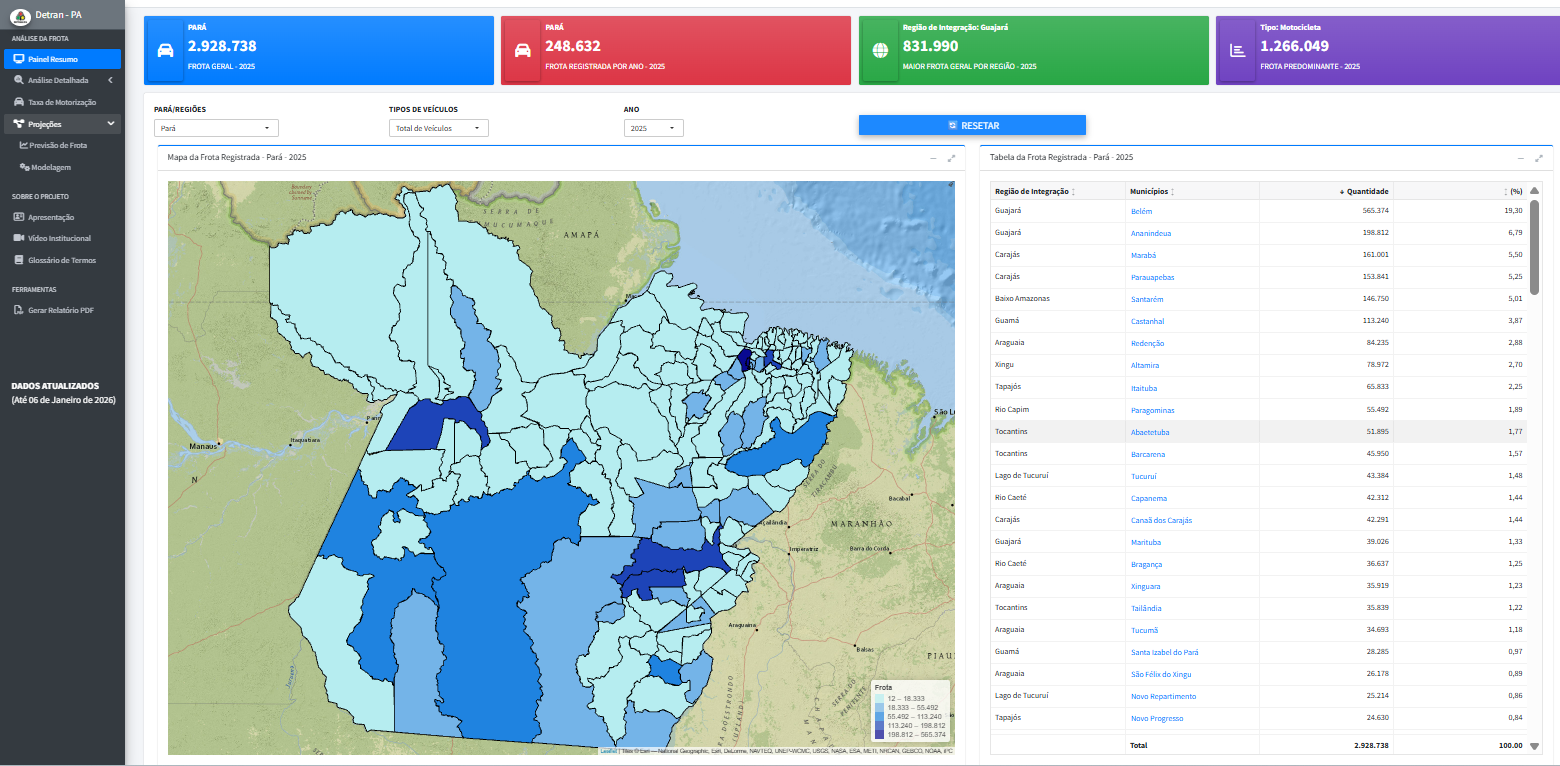
\includegraphics[width=0.8\linewidth]{PainelResumo.png}
    \caption{Aba Principal do \textit{dashboard} desenvolvido em \textit{Shiny}.}
    \label{fig:PainelResumo}
\end{figure}

No painel de Análise Detalhada mostrado na Fig.~\ref{fig:PainelDetalhes}, as tabelas React.js processam matrizes multivariadas (cores, combustíveis, status de circulação, etc.), permitindo agrupamentos sob demanda sem atrasos de rede.

\begin{figure}[!ht]
    \centering
    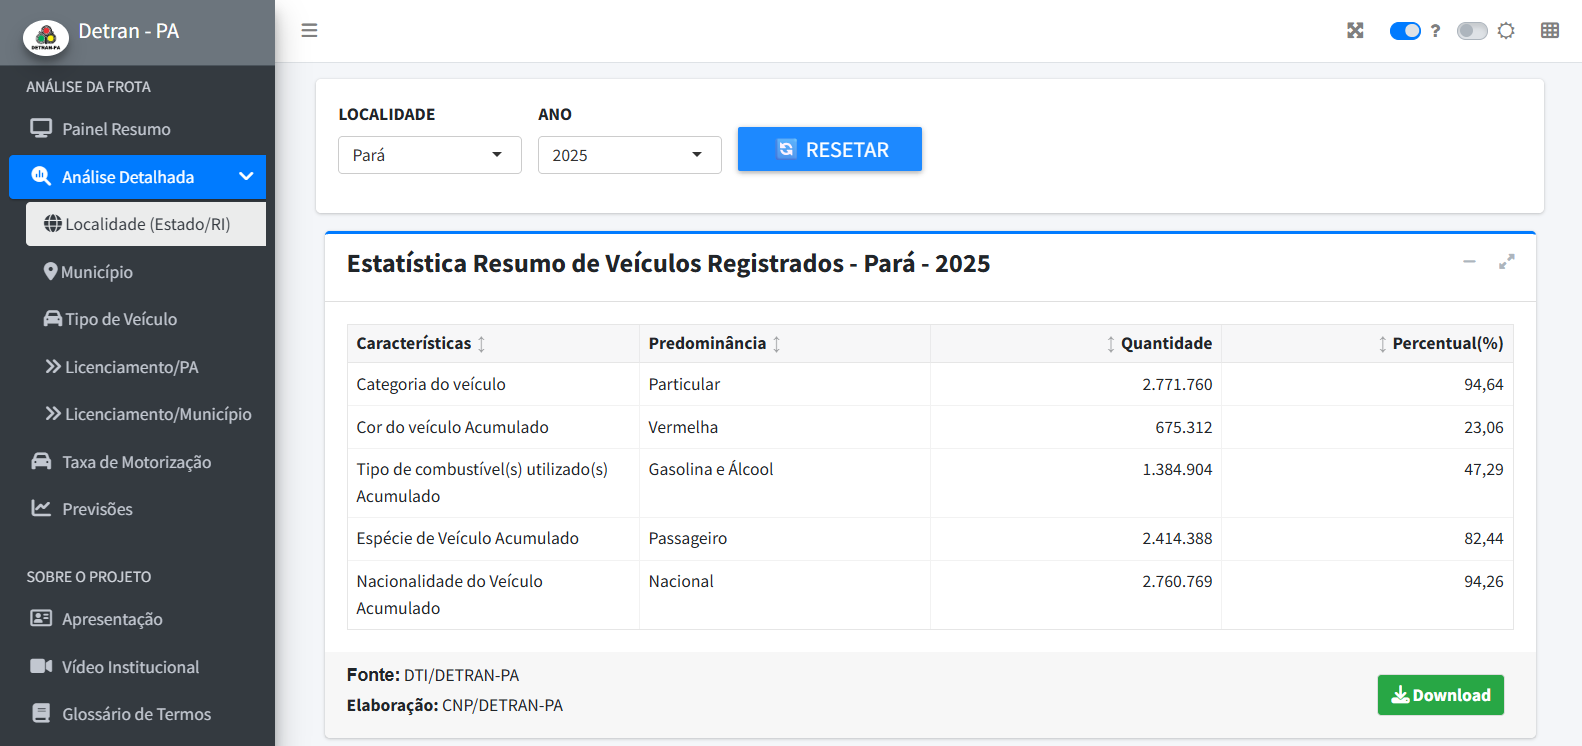
\includegraphics[width=0.95\linewidth]{PainelDetalhes.png}
    \caption{Estatística Resumo sobre os Veículos Registrados.}
    \label{fig:PainelDetalhes}
\end{figure}

A Taxa de Motorização, indicador essencial para engenheiros de trânsito e sociólogos, dimensiona o cruzamento entre densidade veicular e projeções demográficas municipais do IBGE. A Fig.~\ref{fig:GraficoTaxaMotorizacao} exibe a curva de saturação veicular do estado.

\begin{figure}[!ht]
    \centering
    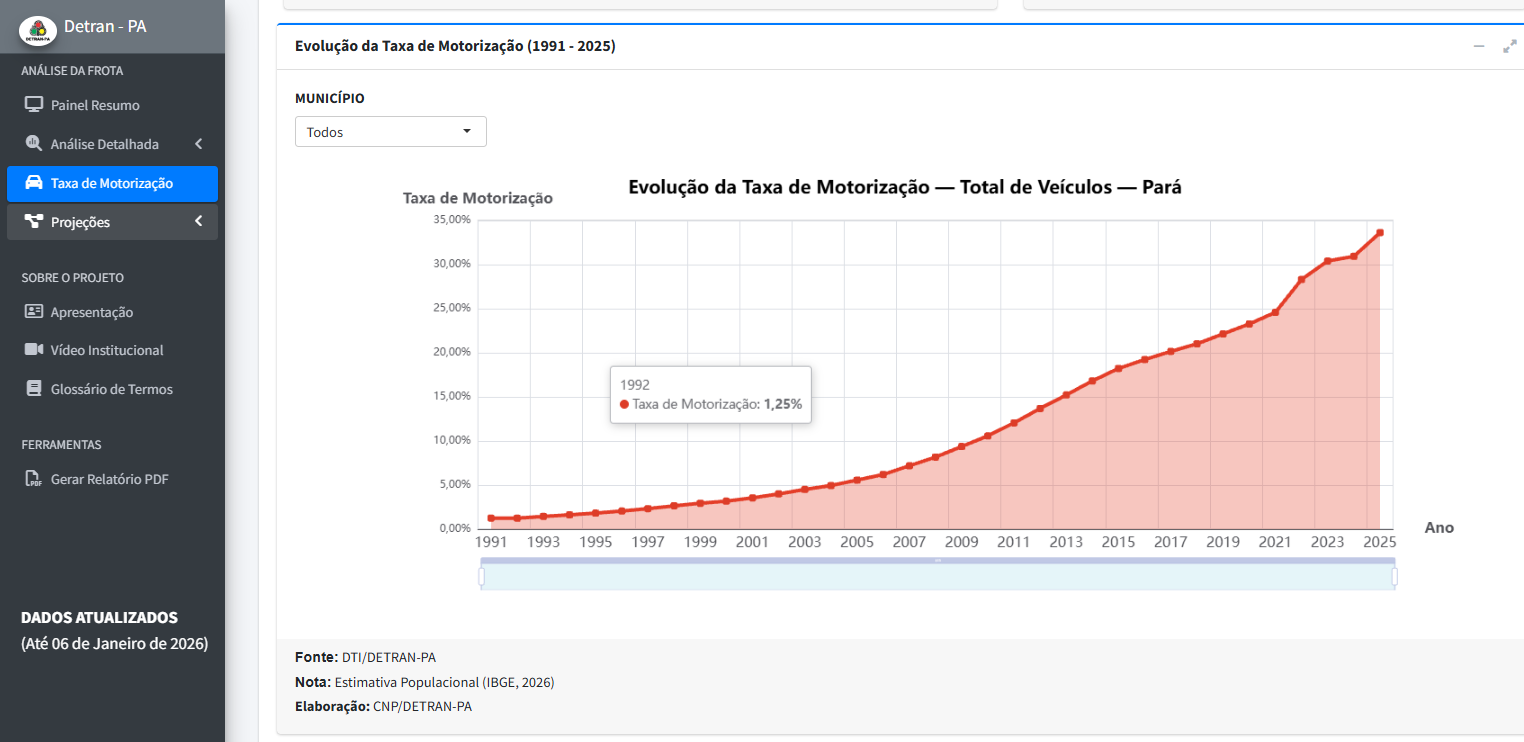
\includegraphics[width=0.95\linewidth]{GraficoTaxaMotorizacao.png}
    \caption{Taxa de Motorização sobre os Veículos Registrados.}
    \label{fig:GraficoTaxaMotorizacao}
\end{figure}


\subsection{Resultados da Modelagem e Avaliação Preditiva}

Para subsidiar tomadas de decisões a longo prazo, o sistema expõe o painel de Previsão Analítica, mostrado na Fig.~\ref{fig:PainelPrevisoes}. Como a arquitetura estipula que a inferência preditiva ocorra de maneira agnóstica na fase de pré-processamento para não onerar o tempo de resposta do \textit{host}, os vetores resultantes até o horizonte temporal de 2.031 foram precalculados, salvos no sistema de arquivos e carregados reativamente no \texttt{Shiny}.

\begin{figure}[!ht]
    \centering
    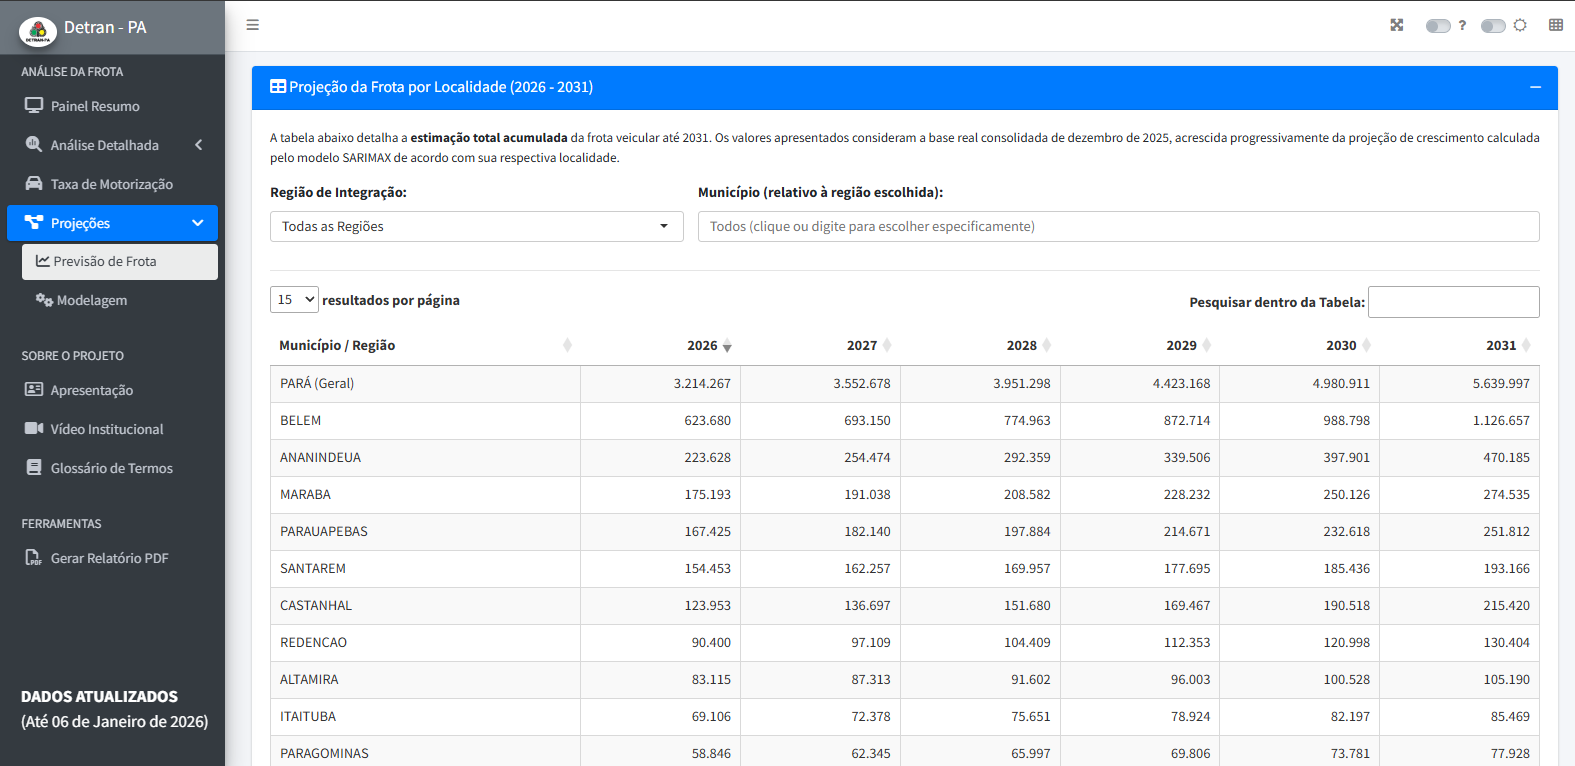
\includegraphics[width=0.95\linewidth]{PainelPrevisoes.png}
    \caption{Painel de Previsões Temporais e Comparação de Modelos}
    \label{fig:PainelPrevisoes}
\end{figure}

\newpage
A acurácia e a estabilidade de convergência dos modelos foram aferidas empregando-se métricas consagradas na literatura de previsão de séries temporais e aprendizado de máquina \cite{hyndman2021forecasting, goodfellow2016deep}. Para avaliar a magnitude dos resíduos e o desvio relativo, calcularam-se o Erro Absoluto Médio (MAE), o Erro Percentual Absoluto Médio (MAPE) e a Raiz do Erro Quadrático Médio (RMSE) \cite{hyndman2021forecasting}, definidos pelas seguintes equações:

$$MAE = \frac{1}{n} \sum_{t=1}^{n} |y_t - \hat{y}_t|$$

$$MAPE = \frac{100\%}{n} \sum_{t=1}^{n} \left| \frac{y_t - \hat{y}_t}{y_t} \right|$$

$$RMSE = \sqrt{\frac{1}{n} \sum_{t=1}^{n} (y_t - \hat{y}_t)^2}$$

Onde $y_t$ representa a contagem real da frota observada no instante $t$, $\hat{y}_t$ é a projeção preditiva correspondente gerada pelos algoritmos e $n$ determina a dimensão temporal da janela de teste. Para mensurar a proporção da variância global explicada pelo modelo, adotou-se o Coeficiente de Determinação ($R^2$) \cite{goodfellow2016deep}:

$$R^2 = 1 - \frac{\sum_{t=1}^{n} (y_t - \hat{y}_t)^2}{\sum_{t=1}^{n} (y_t - \bar{y})^2}$$

Sendo $\bar{y}$ a média global das observações reais da frota. Adicionalmente, para os algoritmos estatísticos (onde a estimativa de máxima verossimilhança é diretamente computável), penalizou-se o excesso de complexidade paramétrica para evitar sobreajuste (\textit{overfitting}) através do Critério de Informação de Akaike (AIC) e do Critério de Informação Bayesiano (BIC) \cite{box1970time, hyndman2021forecasting}:

$$AIC = 2k - 2\ln(\hat{L})$$

$$BIC = k\ln(n) - 2\ln(\hat{L})$$

Em que $k$ representa o número de parâmetros estimados de forma independente pelo modelo e $\hat{L}$ é o valor máximo da função de verossimilhança para o estimador.

Entre os algoritmos estatísticos, o SARIMAX capturou de forma exímia os resíduos sazonais de 12 meses (IPVA) e as quebras estruturais induzidas por instabilidades fiscais anteriores. Ele obteve um MAPE de 5,78\% e coeficiente de determinação global ($R^2$) de 0,7240, o gráfico é mostrado na Fig.~\ref{fig:sarimax}.

\begin{figure}[!ht]
    \centering
    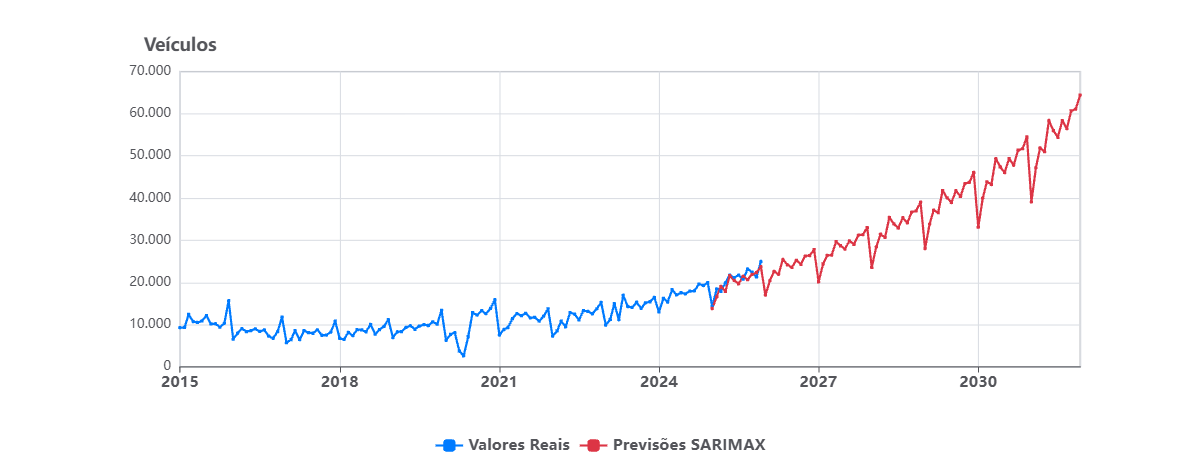
\includegraphics[width=1.1\linewidth]{GraficoSarimax.png}
    \caption{Previsão estatística de crescimento obtida com o modelo SARIMAX.}
    \label{fig:sarimax}
\end{figure}

Nas redes neurais complexas, o cenário difere. O LSTM enfrentou o clássico dilema da explosão de gradiente com dados escassos, gerando alta dispersão. Entretanto, a otimização algorítmica e topológica executada sobre o GRU, embasada no Tensor Global Multidimensional (descrito na metodologia), resultou em predições fiéis ao comportamento das curvas, mostrado na Fig.~\ref{fig:gru}.

\begin{figure}[!ht]
    \centering
    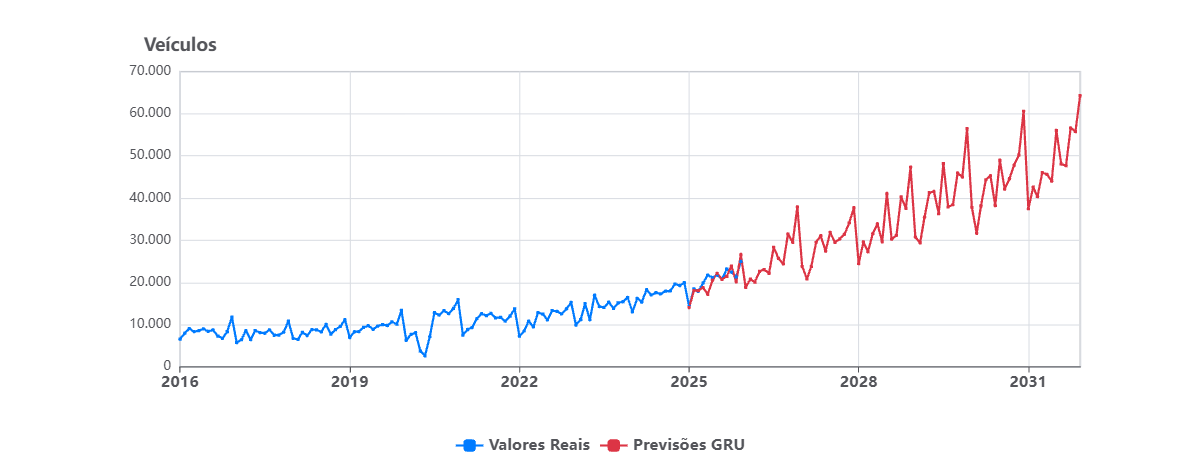
\includegraphics[width=1.1\linewidth]{GraficoGRU.png}
    \caption{Projeção suavizada obtida com a arquitetura tensorial do GRU.}
    \label{fig:gru}
\end{figure}

Os algoritmos foram validados com uma janela de teste de 12 meses no final do treinamento. As métricas comparativas consolidadas de validação (\textit{test-set evaluation}) entre as metodologias testadas estão expostas na Tabela~\ref{tab:comparacao_modelos}.


\newpage
\begin{table}[!ht]
\renewcommand{\arraystretch}{1.3}
\centering
\caption{Comparação das métricas de desempenho no conjunto de validação dos modelos testados.}
\label{tab:comparacao_modelos}
\resizebox{\columnwidth}{!}{%
\begin{tabular}{l|c|c|c|c|c|c}
\hline \hline
\textbf{Modelo} & \textbf{MAPE} & \textbf{MAE} & \textbf{RMSE} & \textbf{AIC} & \textbf{BIC} & \textbf{$R^2$} \\
\hline \hline
LSTM    & 9,07 & 1,803 & 2,292 & 189,70 & 190,67 & 0,2581 \\
GRU     & \textbf{5,19} & \textbf{1,129} & 1,634 & 181,57 & 182,54 & 0,6230 \\
ARIMA   & 9,18 & 1,855 & 2,203 & 188,74 & 189,71 & 0,3150 \\
SARIMA  & 6,75 & 1,406 & 1,660 & 181,94 & 182,91 & 0,6111 \\
SARIMAX & 5,78 & 1,198 & \textbf{1,398} & \textbf{177,83} & \textbf{178,80} & \textbf{0,7240} \\
\hline \hline
\end{tabular}%
}
\end{table}

A eficácia do algoritmo GRU evidenciou-se na obtenção do menor erro da rodada ($MAPE = 5,19\%$). Sua matriz simplificada de dois gates reduziu o montante paramétrico que necessitava ser aprendido, tornando-se imune ao \textit{overfitting}. 

A engenharia preditiva combinada (mais de 140 municípios versus 84 meses efetivos) alimentou a rede neural com mais de 12 mil exemplos de treinamento, viabilizando o entendimento do crescimento como um tecido interligado. 

Em suma, ambos os modelos de ponta (SARIMAX para variância explicada e GRU para mitigação de erro absoluto) apontaram para o mesmo limiar logístico: um acréscimo explosivo de cerca de 60 mil novos veículos circulantes anualmente, saturando a infraestrutura das principais rodovias estaduais até 2031.

Do ponto de vista governamental, o acréscimo contínuo estimado e evidenciado pelos modelos preditivos na ordem de milhares de veículos gera consequências sistêmicas de amplo aspecto. Em primeira instância, o aumento acentuado da taxa de motorização acende o alerta para o esgotamento do planejamento urbano contemporâneo, pressionando diretamente as pastas governamentais a remodelar a estrutura rodoviária, semafórica e ampliar fortemente a disponibilidade de modais multimodais eficientes.

A capacidade do algoritmo de Deep Learning (GRU) de atuar em rede com dados transversais e alcançar um erro marginal de apenas 5\% transforma-o num ativo crucial de inteligência institucional. Paralelamente, prever com precisão a malha veicular permite à secretaria estadual de fazenda estimar, em níveis muito granulares, a arrecadação trilionária de licenciamentos e IPVA ao longo da década, alinhando despesas públicas a receitas fidedignas. O rigor estocástico garantido pelo SARIMAX isolando o choque econômico reitera a tese de que soluções algorítmicas conjuntas (ensemble thinking) são indispensáveis em análises estatais complexas.

Ao converter tais fluxos matemáticos intrincados em um Dashboard Shiny aberto e relatórios Quarto dinâmicos gerados em segundos, o órgão de trânsito não apenas extinguiu o processamento manual moroso dos setores de estatística, mas materializou o espírito central da Lei de Acesso à Informação. Trata-se do rompimento do sigilo burocrático e da ascensão de uma era onde a sociedade civil, a academia e o gestor visualizam assincronamente as mesmas inferências tecnológicas, promovendo uma fiscalização cidadã em larga escala sobre a evolução estrutural e os padrões de mobilidade da sua própria região.


\section{Considerações e Trabalhos Futuros}
\label{sec:conclui}

Este trabalho propôs, implementou e validou uma arquitetura analítica escalável e reprodutível orientada à transparência ativa dos dados de trânsito de um estado brasileiro. O arcabouço construído sob a linguagem R consolidou metodologias díspares de forma harmoniosa: consultas lazy em gigabytes de dados operadas via Apache Arrow, interatividade fluida orquestrada pelo reator web do Shiny, e editoração científica em LaTeX/Quarto de alta fidelidade entregue sem sobrecargas operacionais ao usuário final. 

Na série preditiva, a orquestração do processamento tensorial de dados regionais permitiu que as Redes Neurais Recorrentes (GRU) alcançassem desempenho comparável aos algoritmos clássicos em termos de acurácia, mesmo com a quantidade de dados subótima para o desempenho do modelo, mitigando os desafios de escassez histórica de municípios menores. Do lado da Engenharia de Software, a estabilização do ecossistema via contêineres e topologia de alta disponibilidade no Kubernetes demonstra que ferramentas \textit{open-source} de \textit{Data Science} possuem absoluta robustez para sustentar sistemas de alto tráfego em governos.

Para trabalhos futuros, o horizonte natural desta arquitetura caminha em direção ao monitoramento contínuo da letalidade e sinistralidade de trânsito. Planeja-se a migração da arquitetura estática de banco relacional para uma infraestrutura de mensageria assíncrona, incorporando o \textit{Apache Kafka} para realizar inferências preditivas via stream processing (processamento em tempo real de acidentes e infrações). Essa evolução técnica alavancará a capacidade do Estado de realizar bloqueios rodoviários e operações táticas balizadas em predições baseadas em dados vivos e geolocalizados de mobilidade urbana.


% ================ SEÇÕES EXIGIDAS PELO TEMPLATE ================

\section*{Agradecimentos}
Aos órgãos de fomento à pesquisa e às equipes de tecnologia que disponibilizaram a base de dados anonimizada necessária para o desenvolvimento da plataforma.

\newpage
\section*{Declaração sobre uso de Inteligência Artificial}
Declaro que ferramentas de Inteligência Artificial Generativa foram utilizadas neste trabalho nas seguintes etapas: Grandes Modelos de Linguagem (LLMs) foram utilizados para a revisão ortográfica e gramatical do texto, na etapa de escrita final do artigo. Todo o conteúdo gerado foi revisado criticamente e validado pelo autor, que assume integral responsabilidade pela originalidade e veracidade do texto final, em conformidade com a Portaria CNPq n° 2.664/2026.

% ===================== REFERÊNCIAS =====================

\bibliographystyle{IEEEtran}
\bibliography{referencias} % Certifique-se de que o arquivo referencias.bib está na mesma pasta

\end{document}